\documentclass[11pt,a4paper]{article}
\usepackage[utf8]{inputenc}
\usepackage[T1]{fontenc}
\usepackage{amsfonts}
\usepackage[french]{babel}
\frenchbsetup{StandardLists=true} % à inclure si on utilise \usepackage[francais]{babel}
\usepackage{enumitem}
\usepackage{amssymb}
\usepackage{amsmath}
\usepackage[left=2cm,right=2cm,top=2cm,bottom=2cm]{geometry}
\usepackage{multirow}
\usepackage[dvipsnames]{xcolor}

\usepackage[T1]{fontenc}
\usepackage{fouriernc}
\usepackage{graphicx}

\usepackage{setspace}
\singlespacing

\usepackage{pstricks}
\usepackage{xkeyval}
\usepackage{pst-labo}


\usepackage{multicol}
\usepackage{caption}
\usepackage{fancyhdr}
\pagestyle{fancy}
\renewcommand\headrulewidth{1pt}
\fancyhead[L]{Lycée Denis Diderot }
\fancyhead[R]{Classe de 1 Bac Pro }
\setcounter{page}{17}\fancyfoot[C]{page \thepage}
\fancyfoot[R]{Année 2024-2025}
\fancyfoot[L]{Alexis RUIZ}
\usepackage{multirow,tabularx,booktabs}
\usepackage[tikz]{bclogo} 

\newcommand{\cadreblanc}[1]{%
\medskip\framebox[\linewidth][c]{%
\rule{0mm}{#1mm}}\par
\medskip}

\usepackage{awesomebox}
\setlength{\aweboxvskip}{0mm}
\usepackage{pifont}
\usepackage{chemmacros}
\chemsetup{modules=all}
\setlength{\columnseprule}{.25mm}

\renewcommand{\arraystretch}{2}
\newcommand*\acocher{\quitvmode{\fboxsep0pt \fboxrule0.8pt \fbox{\vrule height1.8ex depth.1ex width0pt \vrule height0pt depth0pt width1.9ex }}}

\newcolumntype{C}[1]{>{\centering\arraybackslash }b{#1}}

\newcommand{\code}{\awesomebox[black]{2pt}{

\includegraphics[scale=0.15]{images/frame.png}
}{black}}

\newcommand{\moteur}{\awesomebox[black]{2pt}{

\includegraphics[scale=1]{images/moteur.jpg} 
}{black}}

\newcommand{\defbox}{\awesomebox[black]{2pt}{
\includegraphics[scale=0.5]{images/appel exam.png}}{black}}

\newcommand{\defconclusion}{\awesomebox[black]{2pt}{\rotatebox{90}{\Large{\textbf{Conclusion}}}}{black}}

  \newenvironment{itemize*}%  % listes compactes
    {\begin{itemize}%
      \setlength{\itemsep}{0pt}%
      \setlength{\parskip}{0pt}}%
    {\end{itemize}}

\frenchbsetup{StandardLists=true}



\begin{document}


\flushleft \textbf{NOM : \hfill Classe : \hspace{3cm} ~~\\[2mm]
Prénom:\\[0,4cm]
}
\hrule\
\\[0,2cm]

\begin{center}
 \LARGE{TP3 - Puissance et énergie d'un feux arrière}
\end{center}

\vspace{3 mm}

\normalsize

\hrule\
\\[0,2cm]
   \begin{center}
   \textbf{Le soin et la rédaction interviendront dans la notation.}
   \end{center} 

\fcolorbox{black}{blue!30}{\textbf{1. Prérequis}} Cocher la (ou les) bonne(s) réponse(s) \\

\begin{itemize}
    \item La tension électrique se mesure en : \\
    \vspace{-5mm} 
        \begin{center}
    \begin{tabular}{C{3cm} C{3cm} C{3cm} C{3cm}}
         $\square$ Ohms & $\square$ Ampères & $\square$ Volts & $\square$ Watts \\
    \end{tabular}
\end{center}

\item L’intensité électrique se mesure en  :\\
\vspace{-5mm} 
        \begin{center}
    \begin{tabular}{C{3cm} C{3cm} C{3cm} C{3cm}}
         $\square$ Ohms & $\square$ Ampères & $\square$ Volts & $\square$ Watts \\
    \end{tabular}
\end{center}


\item La puissance électrique se mesure en : \\
\vspace{-5mm} 
\begin{center}
    \begin{tabular}{C{3cm} C{3cm} C{3cm} C{3cm}}
         $\square$ Joules & $\square$ Ampères & $\square$ Volts & $\square$ Watts \\
    \end{tabular}
\end{center}

\item L’énergie électrique peut s’exprimer en :
\vspace{-5mm} 
\begin{center}
    \begin{tabular}{C{3cm} C{3cm} C{3cm} C{3cm}}
         $\square$ Joules & $\square$ Calories & $\square$ Kilogrammes & $\square$ Wattheures \\
    \end{tabular}
\end{center}

\item La puissance électrique consommée peut se calculer par : 
\vspace{-5mm} 
\begin{center}
    \begin{tabular}{C{3cm} C{3cm} C{3cm} C{3cm}}
         $\square ~~\mathrm{P=U\times I} $  & $\square~~ \mathrm{P = R\times I }$ & $\square ~~\mathrm{P = R\times I^2 } $ & $\square ~~\mathrm{P=E\times t}$\\
    \end{tabular}
\end{center}

\item L’énergie électrique peut se calculer par : 
\vspace{-5mm} 
\begin{center}
    \begin{tabular}{C{3cm} C{3cm} C{3cm} C{3cm}}
         $\square ~~\mathrm{E=U\times I} $  & $\square~~ \mathrm{E = P\times t }$ & $\square ~~\mathrm{E = U\times I \times t } $ & $\square ~~\mathrm{E=I^2\times t}$\\
    \end{tabular}
\end{center}

\end{itemize}

\vspace{2mm}

\fcolorbox{black}{blue!30}{\textbf{2. Protocole}} Proposer un schéma électrique permettant  : d’alimenter le premier filament de la lampe,  de mesurer la tension  aux bornes à ses bornes et de mesurer l’intensité traversant la lampe. \\ 
On utilisera les symboles suivants : \\
\vspace{-5mm}
\begin{center} 
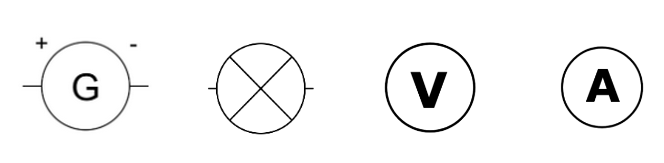
\includegraphics[scale=0.5]{images/instruments.png}
\end{center}
\vspace{-2mm}
\cadreblanc{40}

\newpage

\fcolorbox{black}{blue!30}{\textbf{3. Expérimentation}}

\noindent%
\begin{minipage}{.4\textwidth}%
 \begin{bclogo}[couleur=blue!30 ,  arrondi =0.1 , logo = \bcinfo, epBarre =2]{ Matériel }

\begin{itemize*}
    \item 1 lampe double filament
    \item 1 joule mètre
    \item 1 générateur 12V CC
    \item 7 fils de connexion
\end{itemize*}
\end{bclogo}

\end{minipage}%
\hfill
\begin{minipage}{.5\textwidth}%
\begin{center}
    

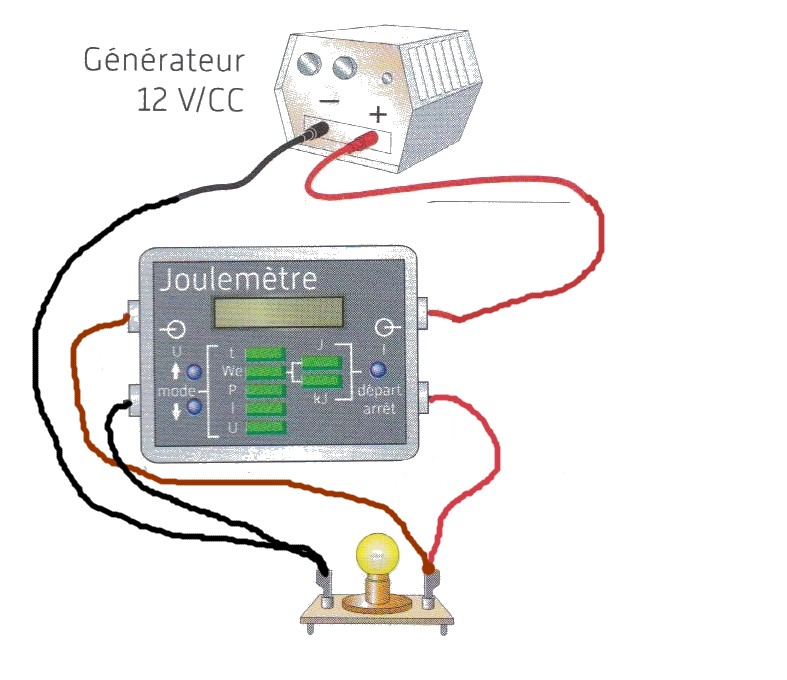
\includegraphics[width=\textwidth]{images/TP1 - Montage.jpg}\end{center}
\end{minipage}%

\begin{enumerate}[label=3.\arabic*]

     \item  Réaliser le montage électrique ci-dessus.
    
\defbox{\fbox{
\begin{minipage}{10cm}{

Appeler M Ruiz pour qu'il vérifie le montage.}

\end{minipage}
}}

\vfill 

\begin{multicols}{2}

   \item  Réglez le joulemètre en mode puissance et relevez la valeur de la puissance $\mathrm{P_1}$ reçue par le filament 1 de la lampe allumée. \\
    
    \vspace{3mm}
    \begin{center}
        \vspace{-5mm} 
        \fbox{\Large{$\mathrm{P_1 = ~~~~~~~~~~~~~~~~}$}}
    \end{center}

    \columnbreak
    
 
     \item Réglez le joulemètre en mode puissance et relevez la valeur de la puissance $\mathrm{P_2}$ reçue par le filament 2 de la lampe allumée. \\
    
    \vspace{3mm}
    \begin{center}
        \vspace{-5mm} 
        \fbox{\Large{$\mathrm{P_2 = ~~~~~~~~~~~~~~~~}$}}
    \end{center}

  \end{multicols}   

  \vfill 

  
\defbox{\fbox{
\begin{minipage}{14cm}{


 Appeler M Ruiz et proposer à l'oral un montage pour mesurer la puissance reçue par la lampe \textbf{avec les deux filaments allumés}.}

\end{minipage}
}}

\vfill 


     \item  Réglez le joulemètre en mode puissance et relevez la valeur de la puissance $\mathrm{P}$ reçue par les filaments 1 \& 2 de la lampe allumée. \\
    
    \vspace{3mm}
    \begin{center}
        \vspace{-5mm} 
        \fbox{\Large{$\mathrm{P = ~~~~~~~~~~~~~~~~ }$}}
    \end{center}

    \item  Proposer une relation liant $\mathrm{P,~~ P_1 ~~et~~ P_2}$ \\ 

    \begin{center}
        \begin{minipage}{5cm}
        \cadreblanc{10}
        \end{minipage}
    \end{center}










    
   \item Réglez le joulemètre en mode énergie et relevez la valeur de l'énergie $E$ reçue par la lampe avec les 2 filaments allumés pour des durées $t$ égales à 60s, 120s, 180s et 240s. \\ Noter les valeurs dans le tableau ci-dessous. 


\begin{center}
    

    \begin{tabular}{|C{2cm}||C{2cm}|C{2cm}|C{2cm}|C{2cm}|}
         \hline
         Durée $t$ (s)& 60 & 120 & 180 & 240\\
         \hline
         Énergie (J)&  &  &  & \\
         \hline
    \end{tabular}
\end{center}

\newpage

     \item  Tracer la représentation graphique modélisant l'énergie mesurée $E$ en $J$ en fonction du temps $t$~en~$s$ \\[1.5 cm]

\begin{center}
    




\begin{tikzpicture}[scale=1]
%papier milli
\draw [very thin, gray!20] (0,-3) grid[step=0.1] (13,10);

\draw [very thin, black!20] (0,-3) grid[step=0.5] (13,10);
\draw [very thin, black!40] (0,-3) grid[step=1] (13,10);
\draw[->,>=stealth] (0,-3) -- (13.5,-3) node[below right] {t(s)};
%stealth définit un style de flèche, "furtif"
\draw[->,>=stealth] (0,-3) -- (0,10.2)node[below left] {E(J)};

\draw (0,-2.9) -- (0,-3.1) node [below left] {{\scriptsize 0}}; 
\draw (3,-2.9) -- (3,-3.1) node [below left] {{\scriptsize 60}}; %échelle abscisse
\draw (0.1,-1) -- (-0.1,-1) node [left] {{\scriptsize 
1000}}; %échelle ordonnée

\end{tikzpicture}
\end{center}

\end{enumerate}




\vfill 

\fcolorbox{black}{blue!30}{\textbf{4. Interprétation }} \\[5mm]
4.1.  En utilisant la dernière colonne de votre tableau de la question 3.6, calculer, en Watt, la puissance reçue par la lampe. \\
\cadreblanc{15}
4.2.  Cette valeur est-elle en accord avec celle mesurée à à la question 3.4. ? \\
\cadreblanc{10}
4.3.  Proposer une relation liant \textbf{l'énergie totale} reçue par la lampe ; \textbf{l'énergie} reçue par le filament 1 et \textbf{l'énergie} reçue par le filament 2.   \\
\cadreblanc{10}


\vfill 


\end{document}